\documentclass[1p]{elsarticle_modified}
%\bibliographystyle{elsarticle-num}

%\usepackage[colorlinks]{hyperref}
%\usepackage{abbrmath_seonhwa} %\Abb, \Ascr, \Acal ,\Abf, \Afrak
\usepackage{amsfonts}
\usepackage{amssymb}
\usepackage{amsmath}
\usepackage{amsthm}
\usepackage{scalefnt}
\usepackage{amsbsy}
\usepackage{kotex}
\usepackage{caption}
\usepackage{subfig}
\usepackage{color}
\usepackage{graphicx}
\usepackage{xcolor} %% white, black, red, green, blue, cyan, magenta, yellow
\usepackage{float}
\usepackage{setspace}
\usepackage{hyperref}

\usepackage{tikz}
\usetikzlibrary{arrows}

\usepackage{multirow}
\usepackage{array} % fixed length table
\usepackage{hhline}

%%%%%%%%%%%%%%%%%%%%%
\makeatletter
\renewcommand*\env@matrix[1][\arraystretch]{%
	\edef\arraystretch{#1}%
	\hskip -\arraycolsep
	\let\@ifnextchar\new@ifnextchar
	\array{*\c@MaxMatrixCols c}}
\makeatother %https://tex.stackexchange.com/questions/14071/how-can-i-increase-the-line-spacing-in-a-matrix
%%%%%%%%%%%%%%%

\usepackage[normalem]{ulem}

\newcommand{\msout}[1]{\ifmmode\text{\sout{\ensuremath{#1}}}\else\sout{#1}\fi}
%SOURCE: \msout is \stkout macro in https://tex.stackexchange.com/questions/20609/strikeout-in-math-mode

\newcommand{\cancel}[1]{
	\ifmmode
	{\color{red}\msout{#1}}
	\else
	{\color{red}\sout{#1}}
	\fi
}

\newcommand{\add}[1]{
	{\color{blue}\uwave{#1}}
}

\newcommand{\replace}[2]{
	\ifmmode
	{\color{red}\msout{#1}}{\color{blue}\uwave{#2}}
	\else
	{\color{red}\sout{#1}}{\color{blue}\uwave{#2}}
	\fi
}

\newcommand{\Sol}{\mathcal{S}} %segment
\newcommand{\D}{D} %diagram
\newcommand{\A}{\mathcal{A}} %arc


%%%%%%%%%%%%%%%%%%%%%%%%%%%%%5 test

\def\sl{\operatorname{\textup{SL}}(2,\Cbb)}
\def\psl{\operatorname{\textup{PSL}}(2,\Cbb)}
\def\quan{\mkern 1mu \triangleright \mkern 1mu}

\theoremstyle{definition}
\newtheorem{thm}{Theorem}[section]
\newtheorem{prop}[thm]{Proposition}
\newtheorem{lem}[thm]{Lemma}
\newtheorem{ques}[thm]{Question}
\newtheorem{cor}[thm]{Corollary}
\newtheorem{defn}[thm]{Definition}
\newtheorem{exam}[thm]{Example}
\newtheorem{rmk}[thm]{Remark}
\newtheorem{alg}[thm]{Algorithm}

\newcommand{\I}{\sqrt{-1}}
\begin{document}

%\begin{frontmatter}
%
%\title{Boundary parabolic representations of knots up to 8 crossings}
%
%%% Group authors per affiliation:
%\author{Yunhi Cho} 
%\address{Department of Mathematics, University of Seoul, Seoul, Korea}
%\ead{yhcho@uos.ac.kr}
%
%
%\author{Seonhwa Kim} %\fnref{s_kim}}
%\address{Center for Geometry and Physics, Institute for Basic Science, Pohang, 37673, Korea}
%\ead{ryeona17@ibs.re.kr}
%
%\author{Hyuk Kim}
%\address{Department of Mathematical Sciences, Seoul National University, Seoul 08826, Korea}
%\ead{hyukkim@snu.ac.kr}
%
%\author{Seokbeom Yoon}
%\address{Department of Mathematical Sciences, Seoul National University, Seoul, 08826,  Korea}
%\ead{sbyoon15@snu.ac.kr}
%
%\begin{abstract}
%We find all boundary parabolic representation of knots up to 8 crossings.
%
%\end{abstract}
%\begin{keyword}
%    \MSC[2010] 57M25 
%\end{keyword}
%
%\end{frontmatter}

%\linenumbers
%\tableofcontents
%
\newcommand\colored[1]{\textcolor{white}{\rule[-0.35ex]{0.8em}{1.4ex}}\kern-0.8em\color{red} #1}%
%\newcommand\colored[1]{\textcolor{white}{ #1}\kern-2.17ex	\textcolor{white}{ #1}\kern-1.81ex	\textcolor{white}{ #1}\kern-2.15ex\color{red}#1	}

{\Large $\underline{12a_{0832}~(K12a_{0832})}$}

\setlength{\tabcolsep}{10pt}
\renewcommand{\arraystretch}{1.6}
\vspace{1cm}\begin{tabular}{m{100pt}>{\centering\arraybackslash}m{274pt}}
\multirow{5}{120pt}{
	\centering
	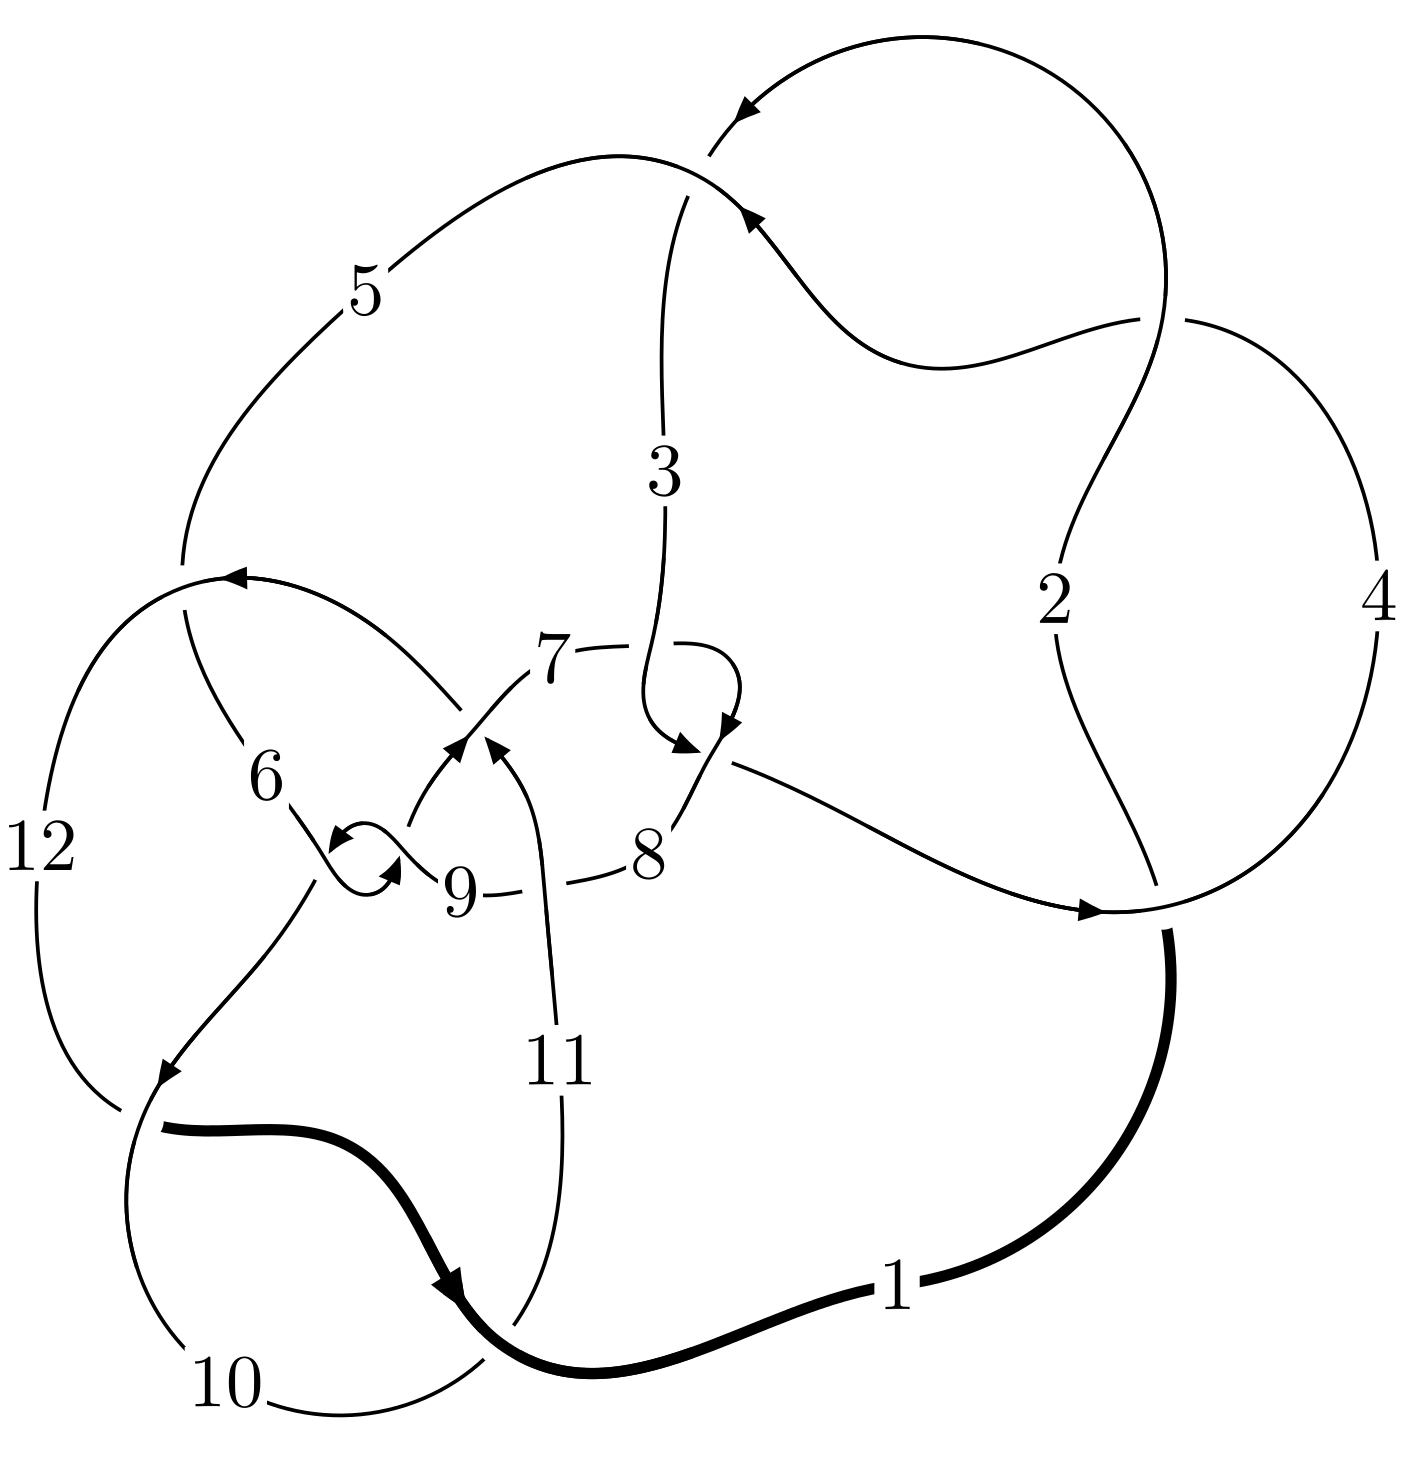
\includegraphics[width=112pt]{../../../GIT/diagram.site/Diagrams/png/1633_12a_0832.png}\\
\ \ \ A knot diagram\footnotemark}&
\allowdisplaybreaks
\textbf{Linearized knot diagam} \\
\cline{2-2}
 &
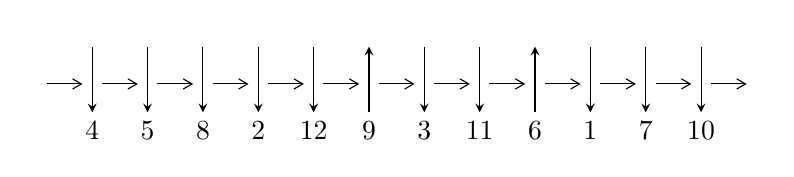
\begin{tikzpicture}[x=20pt, y=17pt]
	% nodes
	\node (C0) at (0, 0) {};
	\node (C1) at (1, 0) {};
	\node (C1U) at (1, +1) {};
	\node (C1D) at (1, -1) {4};

	\node (C2) at (2, 0) {};
	\node (C2U) at (2, +1) {};
	\node (C2D) at (2, -1) {5};

	\node (C3) at (3, 0) {};
	\node (C3U) at (3, +1) {};
	\node (C3D) at (3, -1) {8};

	\node (C4) at (4, 0) {};
	\node (C4U) at (4, +1) {};
	\node (C4D) at (4, -1) {2};

	\node (C5) at (5, 0) {};
	\node (C5U) at (5, +1) {};
	\node (C5D) at (5, -1) {12};

	\node (C6) at (6, 0) {};
	\node (C6U) at (6, +1) {};
	\node (C6D) at (6, -1) {9};

	\node (C7) at (7, 0) {};
	\node (C7U) at (7, +1) {};
	\node (C7D) at (7, -1) {3};

	\node (C8) at (8, 0) {};
	\node (C8U) at (8, +1) {};
	\node (C8D) at (8, -1) {11};

	\node (C9) at (9, 0) {};
	\node (C9U) at (9, +1) {};
	\node (C9D) at (9, -1) {6};

	\node (C10) at (10, 0) {};
	\node (C10U) at (10, +1) {};
	\node (C10D) at (10, -1) {1};

	\node (C11) at (11, 0) {};
	\node (C11U) at (11, +1) {};
	\node (C11D) at (11, -1) {7};

	\node (C12) at (12, 0) {};
	\node (C12U) at (12, +1) {};
	\node (C12D) at (12, -1) {10};
	\node (C13) at (13, 0) {};

	% arrows
	\draw[->,>={angle 60}]
	(C0) edge (C1) (C1) edge (C2) (C2) edge (C3) (C3) edge (C4) (C4) edge (C5) (C5) edge (C6) (C6) edge (C7) (C7) edge (C8) (C8) edge (C9) (C9) edge (C10) (C10) edge (C11) (C11) edge (C12) (C12) edge (C13) ;	\draw[->,>=stealth]
	(C1U) edge (C1D) (C2U) edge (C2D) (C3U) edge (C3D) (C4U) edge (C4D) (C5U) edge (C5D) (C6D) edge (C6U) (C7U) edge (C7D) (C8U) edge (C8D) (C9D) edge (C9U) (C10U) edge (C10D) (C11U) edge (C11D) (C12U) edge (C12D) ;
	\end{tikzpicture} \\
\hhline{~~} \\& 
\textbf{Solving Sequence} \\ \cline{2-2} 
 &
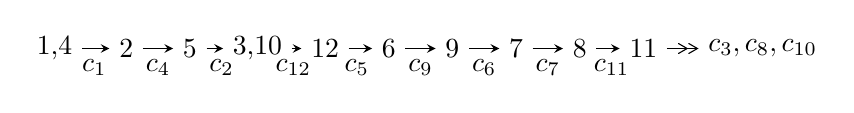
\begin{tikzpicture}[x=23pt, y=7pt]
	% node
	\node (A0) at (-1/8, 0) {1,4};
	\node (A1) at (1, 0) {2};
	\node (A2) at (2, 0) {5};
	\node (A3) at (49/16, 0) {3,10};
	\node (A4) at (33/8, 0) {12};
	\node (A5) at (41/8, 0) {6};
	\node (A6) at (49/8, 0) {9};
	\node (A7) at (57/8, 0) {7};
	\node (A8) at (65/8, 0) {8};
	\node (A9) at (73/8, 0) {11};
	\node (C1) at (1/2, -1) {$c_{1}$};
	\node (C2) at (3/2, -1) {$c_{4}$};
	\node (C3) at (5/2, -1) {$c_{2}$};
	\node (C4) at (29/8, -1) {$c_{12}$};
	\node (C5) at (37/8, -1) {$c_{5}$};
	\node (C6) at (45/8, -1) {$c_{9}$};
	\node (C7) at (53/8, -1) {$c_{6}$};
	\node (C8) at (61/8, -1) {$c_{7}$};
	\node (C9) at (69/8, -1) {$c_{11}$};
	\node (A10) at (11, 0) {$c_{3},c_{8},c_{10}$};

	% edge
	\draw[->,>=stealth]	
	(A0) edge (A1) (A1) edge (A2) (A2) edge (A3) (A3) edge (A4) (A4) edge (A5) (A5) edge (A6) (A6) edge (A7) (A7) edge (A8) (A8) edge (A9) ;
	\draw[->>,>={angle 60}]	
	(A9) edge (A10);
\end{tikzpicture} \\ 

\end{tabular} \\

\footnotetext{
The image of knot diagram is generated by the software ``\textbf{Draw programme}" developed by Andrew Bartholomew(\url{http://www.layer8.co.uk/maths/draw/index.htm\#Running-draw}), where we modified some parts for our purpose(\url{https://github.com/CATsTAILs/LinksPainter}).
}\phantom \\ \newline 
\centering \textbf{Ideals for irreducible components\footnotemark of $X_{\text{par}}$} 
 
\begin{align*}
I^u_{1}&=\langle 
1.82100\times10^{145} u^{106}+1.76856\times10^{146} u^{105}+\cdots+2.34604\times10^{144} b+1.63398\times10^{145},\\
\phantom{I^u_{1}}&\phantom{= \langle  }-9.00860\times10^{144} u^{106}-8.87315\times10^{145} u^{105}+\cdots+3.11583\times10^{143} a-8.18986\times10^{144},\\
\phantom{I^u_{1}}&\phantom{= \langle  }u^{107}+11 u^{106}+\cdots- u+1\rangle \\
I^u_{2}&=\langle 
b^9- b^8-2 b^7+3 b^6+b^5-3 b^4+2 b^3- b+1,\;a-1,\;u-1\rangle \\
I^u_{3}&=\langle 
b+1,\;-12 u^2+17 a-11 u+8,\;u^3+u^2-1\rangle \\
\\
\end{align*}
\raggedright * 3 irreducible components of $\dim_{\mathbb{C}}=0$, with total 119 representations.\\
\footnotetext{All coefficients of polynomials are rational numbers. But the coefficients are sometimes approximated in decimal forms when there is not enough margin.}
\newpage
\renewcommand{\arraystretch}{1}
\centering \section*{I. $I^u_{1}= \langle 1.82\times10^{145} u^{106}+1.77\times10^{146} u^{105}+\cdots+2.35\times10^{144} b+1.63\times10^{145},\;-9.01\times10^{144} u^{106}-8.87\times10^{145} u^{105}+\cdots+3.12\times10^{143} a-8.19\times10^{144},\;u^{107}+11 u^{106}+\cdots- u+1 \rangle$}
\flushleft \textbf{(i) Arc colorings}\\
\begin{tabular}{m{7pt} m{180pt} m{7pt} m{180pt} }
\flushright $a_{1}=$&$\begin{pmatrix}1\\0\end{pmatrix}$ \\
\flushright $a_{4}=$&$\begin{pmatrix}0\\u\end{pmatrix}$ \\
\flushright $a_{2}=$&$\begin{pmatrix}1\\u^2\end{pmatrix}$ \\
\flushright $a_{5}=$&$\begin{pmatrix}- u\\- u^3+u\end{pmatrix}$ \\
\flushright $a_{3}=$&$\begin{pmatrix}- u^2+1\\- u^4+2 u^2\end{pmatrix}$ \\
\flushright $a_{10}=$&$\begin{pmatrix}28.9123 u^{106}+284.776 u^{105}+\cdots-57.4382 u+26.2847\\-7.76201 u^{106}-75.3850 u^{105}+\cdots+12.3022 u-6.96486\end{pmatrix}$ \\
\flushright $a_{12}=$&$\begin{pmatrix}35.3044 u^{106}+346.752 u^{105}+\cdots-60.1629 u+30.1321\\11.0948 u^{106}+107.535 u^{105}+\cdots-11.2109 u+7.50499\end{pmatrix}$ \\
\flushright $a_{6}=$&$\begin{pmatrix}-225.444 u^{106}-2126.33 u^{105}+\cdots+217.402 u-139.053\\-3.47317 u^{106}-15.3113 u^{105}+\cdots-22.8525 u+7.66552\end{pmatrix}$ \\
\flushright $a_{9}=$&$\begin{pmatrix}152.968 u^{106}+1511.32 u^{105}+\cdots-222.234 u+128.653\\85.3954 u^{106}+812.499 u^{105}+\cdots-90.9059 u+55.8114\end{pmatrix}$ \\
\flushright $a_{7}=$&$\begin{pmatrix}-4.74413 u^{106}-45.0876 u^{105}+\cdots+1.45576 u-3.57826\\-1.77398 u^{106}-16.9646 u^{105}+\cdots+0.374396 u-0.558079\end{pmatrix}$ \\
\flushright $a_{8}=$&$\begin{pmatrix}4.11969 u^{106}+39.2305 u^{105}+\cdots-8.20858 u+1.92021\\2.41999 u^{106}+24.9542 u^{105}+\cdots-5.96901 u+3.00759\end{pmatrix}$ \\
\flushright $a_{11}=$&$\begin{pmatrix}36.6743 u^{106}+360.161 u^{105}+\cdots-69.7404 u+33.2495\\-7.76201 u^{106}-75.3850 u^{105}+\cdots+12.3022 u-6.96486\end{pmatrix}$\\&\end{tabular}
\flushleft \textbf{(ii) Obstruction class $= -1$}\\~\\
\flushleft \textbf{(iii) Cusp Shapes $= -205.058 u^{106}-2014.48 u^{105}+\cdots+295.936 u-174.019$}\\~\\
\newpage\renewcommand{\arraystretch}{1}
\flushleft \textbf{(iv) u-Polynomials at the component}\newline \\
\begin{tabular}{m{50pt}|m{274pt}}
Crossings & \hspace{64pt}u-Polynomials at each crossing \\
\hline $$\begin{aligned}c_{1},c_{2},c_{4}\end{aligned}$$&$\begin{aligned}
&u^{107}-11 u^{106}+\cdots- u-1
\end{aligned}$\\
\hline $$\begin{aligned}c_{3},c_{7}\end{aligned}$$&$\begin{aligned}
&u^{107}-2 u^{106}+\cdots-512 u+512
\end{aligned}$\\
\hline $$\begin{aligned}c_{5}\end{aligned}$$&$\begin{aligned}
&17(17 u^{107}+96 u^{106}+\cdots-2.67194\times10^{8} u+4.35330\times10^{7})
\end{aligned}$\\
\hline $$\begin{aligned}c_{6},c_{9}\end{aligned}$$&$\begin{aligned}
&u^{107}+3 u^{106}+\cdots-3 u-1
\end{aligned}$\\
\hline $$\begin{aligned}c_{8}\end{aligned}$$&$\begin{aligned}
&17(17 u^{107}+61 u^{106}+\cdots+4.98410\times10^{7} u-2813417)
\end{aligned}$\\
\hline $$\begin{aligned}c_{10},c_{12}\end{aligned}$$&$\begin{aligned}
&u^{107}-5 u^{106}+\cdots-5466 u-289
\end{aligned}$\\
\hline $$\begin{aligned}c_{11}\end{aligned}$$&$\begin{aligned}
&u^{107}+2 u^{106}+\cdots-10404 u+2312
\end{aligned}$\\
\hline
\end{tabular}\\~\\
\newpage\renewcommand{\arraystretch}{1}
\flushleft \textbf{(v) Riley Polynomials at the component}\newline \\
\begin{tabular}{m{50pt}|m{274pt}}
Crossings & \hspace{64pt}Riley Polynomials at each crossing \\
\hline $$\begin{aligned}c_{1},c_{2},c_{4}\end{aligned}$$&$\begin{aligned}
&y^{107}-99 y^{106}+\cdots-29 y-1
\end{aligned}$\\
\hline $$\begin{aligned}c_{3},c_{7}\end{aligned}$$&$\begin{aligned}
&y^{107}-54 y^{106}+\cdots+7340032 y-262144
\end{aligned}$\\
\hline $$\begin{aligned}c_{5}\end{aligned}$$&$\begin{aligned}
&289(289 y^{107}-19076 y^{106}+\cdots+8.77063\times10^{16} y-1.89512\times10^{15})
\end{aligned}$\\
\hline $$\begin{aligned}c_{6},c_{9}\end{aligned}$$&$\begin{aligned}
&y^{107}+73 y^{106}+\cdots+55 y-1
\end{aligned}$\\
\hline $$\begin{aligned}c_{8}\end{aligned}$$&$\begin{aligned}
&289\\
&\cdot(289 y^{107}-7971 y^{106}+\cdots+1153422073109755 y-7915315215889)
\end{aligned}$\\
\hline $$\begin{aligned}c_{10},c_{12}\end{aligned}$$&$\begin{aligned}
&y^{107}-81 y^{106}+\cdots+6093612 y-83521
\end{aligned}$\\
\hline $$\begin{aligned}c_{11}\end{aligned}$$&$\begin{aligned}
&y^{107}-18 y^{106}+\cdots+277740560 y-5345344
\end{aligned}$\\
\hline
\end{tabular}\\~\\
\newpage\flushleft \textbf{(vi) Complex Volumes and Cusp Shapes}
$$\begin{array}{c|c|c}  
\text{Solutions to }I^u_{1}& \I (\text{vol} + \sqrt{-1}CS) & \text{Cusp shape}\\
 \hline 
\begin{aligned}
u &= \phantom{-}0.346089 + 0.926510 I \\
a &= \phantom{-}0.488603 - 1.149700 I \\
b &= \phantom{-}1.44877 + 0.53359 I\end{aligned}
 & -7.4189 - 13.7965 I & \phantom{-0.000000 } 0 \\ \hline\begin{aligned}
u &= \phantom{-}0.346089 - 0.926510 I \\
a &= \phantom{-}0.488603 + 1.149700 I \\
b &= \phantom{-}1.44877 - 0.53359 I\end{aligned}
 & -7.4189 + 13.7965 I & \phantom{-0.000000 } 0 \\ \hline\begin{aligned}
u &= \phantom{-}0.369955 + 0.942148 I \\
a &= \phantom{-}0.573386 - 0.891132 I \\
b &= \phantom{-}1.249130 + 0.376668 I\end{aligned}
 & -2.55413 - 8.13238 I & \phantom{-0.000000 } 0 \\ \hline\begin{aligned}
u &= \phantom{-}0.369955 - 0.942148 I \\
a &= \phantom{-}0.573386 + 0.891132 I \\
b &= \phantom{-}1.249130 - 0.376668 I\end{aligned}
 & -2.55413 + 8.13238 I & \phantom{-0.000000 } 0 \\ \hline\begin{aligned}
u &= \phantom{-}0.928095 + 0.328024 I \\
a &= \phantom{-}1.067700 - 0.348911 I \\
b &= \phantom{-}0.122990 + 0.398571 I\end{aligned}
 & -0.769990 - 0.237218 I & \phantom{-0.000000 } 0 \\ \hline\begin{aligned}
u &= \phantom{-}0.928095 - 0.328024 I \\
a &= \phantom{-}1.067700 + 0.348911 I \\
b &= \phantom{-}0.122990 - 0.398571 I\end{aligned}
 & -0.769990 + 0.237218 I & \phantom{-0.000000 } 0 \\ \hline\begin{aligned}
u &= \phantom{-}0.319909 + 1.003060 I \\
a &= \phantom{-}0.300455 - 0.534456 I \\
b &= \phantom{-}1.246370 + 0.010174 I\end{aligned}
 & -6.46600 - 1.47782 I & \phantom{-0.000000 } 0 \\ \hline\begin{aligned}
u &= \phantom{-}0.319909 - 1.003060 I \\
a &= \phantom{-}0.300455 + 0.534456 I \\
b &= \phantom{-}1.246370 - 0.010174 I\end{aligned}
 & -6.46600 + 1.47782 I & \phantom{-0.000000 } 0 \\ \hline\begin{aligned}
u &= \phantom{-}0.945816\phantom{ +0.000000I} \\
a &= \phantom{-}2.59957\phantom{ +0.000000I} \\
b &= -0.936011\phantom{ +0.000000I}\end{aligned}
 & -3.02083\phantom{ +0.000000I} & \phantom{-0.000000 } 0 \\ \hline\begin{aligned}
u &= \phantom{-}1.049800 + 0.152492 I \\
a &= \phantom{-}2.59795 + 1.35800 I \\
b &= -1.182570 - 0.120195 I\end{aligned}
 & -5.90093 - 0.77524 I & \phantom{-0.000000 } 0\\
 \hline 
 \end{array}$$\newpage$$\begin{array}{c|c|c}  
\text{Solutions to }I^u_{1}& \I (\text{vol} + \sqrt{-1}CS) & \text{Cusp shape}\\
 \hline 
\begin{aligned}
u &= \phantom{-}1.049800 - 0.152492 I \\
a &= \phantom{-}2.59795 - 1.35800 I \\
b &= -1.182570 + 0.120195 I\end{aligned}
 & -5.90093 + 0.77524 I & \phantom{-0.000000 } 0 \\ \hline\begin{aligned}
u &= \phantom{-}0.771747 + 0.482029 I \\
a &= \phantom{-}1.166080 - 0.347003 I \\
b &= -0.311412 + 1.048800 I\end{aligned}
 & -3.78091 + 2.99219 I & \phantom{-0.000000 } 0 \\ \hline\begin{aligned}
u &= \phantom{-}0.771747 - 0.482029 I \\
a &= \phantom{-}1.166080 + 0.347003 I \\
b &= -0.311412 - 1.048800 I\end{aligned}
 & -3.78091 - 2.99219 I & \phantom{-0.000000 } 0 \\ \hline\begin{aligned}
u &= -0.828331 + 0.756192 I \\
a &= \phantom{-}0.891464 + 0.459958 I \\
b &= \phantom{-}1.003920 - 0.044300 I\end{aligned}
 & \phantom{-}1.38178 + 2.91494 I & \phantom{-0.000000 } 0 \\ \hline\begin{aligned}
u &= -0.828331 - 0.756192 I \\
a &= \phantom{-}0.891464 - 0.459958 I \\
b &= \phantom{-}1.003920 + 0.044300 I\end{aligned}
 & \phantom{-}1.38178 - 2.91494 I & \phantom{-0.000000 } 0 \\ \hline\begin{aligned}
u &= \phantom{-}0.343042 + 0.788869 I \\
a &= -0.336263 + 0.963037 I \\
b &= -0.149645 - 1.288650 I\end{aligned}
 & -2.37272 - 7.54825 I & \phantom{-0.000000 } 0 \\ \hline\begin{aligned}
u &= \phantom{-}0.343042 - 0.788869 I \\
a &= -0.336263 - 0.963037 I \\
b &= -0.149645 + 1.288650 I\end{aligned}
 & -2.37272 + 7.54825 I & \phantom{-0.000000 } 0 \\ \hline\begin{aligned}
u &= \phantom{-}0.922174 + 0.690097 I \\
a &= \phantom{-}0.581180 - 0.416925 I \\
b &= \phantom{-}1.43011 - 0.44307 I\end{aligned}
 & -9.14754 + 8.24261 I & \phantom{-0.000000 } 0 \\ \hline\begin{aligned}
u &= \phantom{-}0.922174 - 0.690097 I \\
a &= \phantom{-}0.581180 + 0.416925 I \\
b &= \phantom{-}1.43011 + 0.44307 I\end{aligned}
 & -9.14754 - 8.24261 I & \phantom{-0.000000 } 0 \\ \hline\begin{aligned}
u &= \phantom{-}0.448171 + 0.709899 I \\
a &= -0.18414 + 1.45497 I \\
b &= -1.55514 - 0.73695 I\end{aligned}
 & -6.91732 - 4.41662 I & \phantom{-0.000000 } 0\\
 \hline 
 \end{array}$$\newpage$$\begin{array}{c|c|c}  
\text{Solutions to }I^u_{1}& \I (\text{vol} + \sqrt{-1}CS) & \text{Cusp shape}\\
 \hline 
\begin{aligned}
u &= \phantom{-}0.448171 - 0.709899 I \\
a &= -0.18414 - 1.45497 I \\
b &= -1.55514 + 0.73695 I\end{aligned}
 & -6.91732 + 4.41662 I & \phantom{-0.000000 } 0 \\ \hline\begin{aligned}
u &= \phantom{-}0.557495 + 0.610684 I \\
a &= \phantom{-}0.362867 + 0.478199 I \\
b &= -1.65203 + 0.47475 I\end{aligned}
 & -7.33756 - 0.07613 I & \phantom{-0.000000 } 0 \\ \hline\begin{aligned}
u &= \phantom{-}0.557495 - 0.610684 I \\
a &= \phantom{-}0.362867 - 0.478199 I \\
b &= -1.65203 - 0.47475 I\end{aligned}
 & -7.33756 + 0.07613 I & \phantom{-0.000000 } 0 \\ \hline\begin{aligned}
u &= \phantom{-}0.759499 + 0.321795 I \\
a &= \phantom{-}1.330620 + 0.358278 I \\
b &= -0.378863 - 0.498684 I\end{aligned}
 & -3.58750 - 2.31232 I & \phantom{-0.000000 } 0 \\ \hline\begin{aligned}
u &= \phantom{-}0.759499 - 0.321795 I \\
a &= \phantom{-}1.330620 - 0.358278 I \\
b &= -0.378863 + 0.498684 I\end{aligned}
 & -3.58750 + 2.31232 I & \phantom{-0.000000 } 0 \\ \hline\begin{aligned}
u &= \phantom{-}0.289663 + 0.766909 I \\
a &= \phantom{-}0.002340 + 0.697636 I \\
b &= \phantom{-}0.077224 - 0.771549 I\end{aligned}
 & \phantom{-}1.09835 - 3.92237 I & \phantom{-0.000000 } 0 \\ \hline\begin{aligned}
u &= \phantom{-}0.289663 - 0.766909 I \\
a &= \phantom{-}0.002340 - 0.697636 I \\
b &= \phantom{-}0.077224 + 0.771549 I\end{aligned}
 & \phantom{-}1.09835 + 3.92237 I & \phantom{-0.000000 } 0 \\ \hline\begin{aligned}
u &= \phantom{-}0.926197 + 0.743885 I \\
a &= \phantom{-}0.720813 - 0.394658 I \\
b &= \phantom{-}1.217190 - 0.229736 I\end{aligned}
 & -4.18081 + 2.37986 I & \phantom{-0.000000 } 0 \\ \hline\begin{aligned}
u &= \phantom{-}0.926197 - 0.743885 I \\
a &= \phantom{-}0.720813 + 0.394658 I \\
b &= \phantom{-}1.217190 + 0.229736 I\end{aligned}
 & -4.18081 - 2.37986 I & \phantom{-0.000000 } 0 \\ \hline\begin{aligned}
u &= -1.195860 + 0.071246 I \\
a &= \phantom{-}0.834976 + 0.099978 I \\
b &= \phantom{-}1.081680 - 0.553383 I\end{aligned}
 & -5.80226 + 7.40735 I & \phantom{-0.000000 } 0\\
 \hline 
 \end{array}$$\newpage$$\begin{array}{c|c|c}  
\text{Solutions to }I^u_{1}& \I (\text{vol} + \sqrt{-1}CS) & \text{Cusp shape}\\
 \hline 
\begin{aligned}
u &= -1.195860 - 0.071246 I \\
a &= \phantom{-}0.834976 - 0.099978 I \\
b &= \phantom{-}1.081680 + 0.553383 I\end{aligned}
 & -5.80226 - 7.40735 I & \phantom{-0.000000 } 0 \\ \hline\begin{aligned}
u &= -0.319822 + 0.706800 I \\
a &= \phantom{-}0.185472 + 0.770438 I \\
b &= \phantom{-}1.180450 + 0.258145 I\end{aligned}
 & -3.77986 - 4.80948 I & \phantom{-0.000000 } 0 \\ \hline\begin{aligned}
u &= -0.319822 - 0.706800 I \\
a &= \phantom{-}0.185472 - 0.770438 I \\
b &= \phantom{-}1.180450 - 0.258145 I\end{aligned}
 & -3.77986 + 4.80948 I & \phantom{-0.000000 } 0 \\ \hline\begin{aligned}
u &= \phantom{-}1.012440 + 0.691885 I \\
a &= \phantom{-}0.826522 - 0.541378 I \\
b &= \phantom{-}1.304000 + 0.146196 I\end{aligned}
 & -8.58798 - 4.36356 I & \phantom{-0.000000 } 0 \\ \hline\begin{aligned}
u &= \phantom{-}1.012440 - 0.691885 I \\
a &= \phantom{-}0.826522 + 0.541378 I \\
b &= \phantom{-}1.304000 - 0.146196 I\end{aligned}
 & -8.58798 + 4.36356 I & \phantom{-0.000000 } 0 \\ \hline\begin{aligned}
u &= \phantom{-}0.391589 + 0.655721 I \\
a &= -0.43938 + 1.82965 I \\
b &= -1.073250 - 0.329860 I\end{aligned}
 & -2.56341 - 2.94691 I & \phantom{-0.000000 } 0 \\ \hline\begin{aligned}
u &= \phantom{-}0.391589 - 0.655721 I \\
a &= -0.43938 - 1.82965 I \\
b &= -1.073250 + 0.329860 I\end{aligned}
 & -2.56341 + 2.94691 I & \phantom{-0.000000 } 0 \\ \hline\begin{aligned}
u &= \phantom{-}0.316249 + 0.663493 I \\
a &= \phantom{-}1.258330 + 0.584184 I \\
b &= -0.209859 + 0.022387 I\end{aligned}
 & -2.30486 - 1.44330 I & \phantom{-0.000000 } 0 \\ \hline\begin{aligned}
u &= \phantom{-}0.316249 - 0.663493 I \\
a &= \phantom{-}1.258330 - 0.584184 I \\
b &= -0.209859 - 0.022387 I\end{aligned}
 & -2.30486 + 1.44330 I & \phantom{-0.000000 } 0 \\ \hline\begin{aligned}
u &= -1.263060 + 0.081449 I \\
a &= \phantom{-}0.824442 + 0.083550 I \\
b &= \phantom{-}0.727801 - 0.763902 I\end{aligned}
 & -0.72189 + 2.74860 I & \phantom{-0.000000 } 0\\
 \hline 
 \end{array}$$\newpage$$\begin{array}{c|c|c}  
\text{Solutions to }I^u_{1}& \I (\text{vol} + \sqrt{-1}CS) & \text{Cusp shape}\\
 \hline 
\begin{aligned}
u &= -1.263060 - 0.081449 I \\
a &= \phantom{-}0.824442 - 0.083550 I \\
b &= \phantom{-}0.727801 + 0.763902 I\end{aligned}
 & -0.72189 - 2.74860 I & \phantom{-0.000000 } 0 \\ \hline\begin{aligned}
u &= \phantom{-}1.272250 + 0.106081 I \\
a &= \phantom{-}0.98579 + 1.17507 I \\
b &= -0.362733 + 0.158221 I\end{aligned}
 & -4.76982 + 0.36186 I & \phantom{-0.000000 } 0 \\ \hline\begin{aligned}
u &= \phantom{-}1.272250 - 0.106081 I \\
a &= \phantom{-}0.98579 - 1.17507 I \\
b &= -0.362733 - 0.158221 I\end{aligned}
 & -4.76982 - 0.36186 I & \phantom{-0.000000 } 0 \\ \hline\begin{aligned}
u &= \phantom{-}0.451827 + 0.536220 I \\
a &= -0.943034 - 0.499437 I \\
b &= -1.144990 + 0.140910 I\end{aligned}
 & -2.97691 - 0.95326 I & \phantom{-0.000000 } 0 \\ \hline\begin{aligned}
u &= \phantom{-}0.451827 - 0.536220 I \\
a &= -0.943034 + 0.499437 I \\
b &= -1.144990 - 0.140910 I\end{aligned}
 & -2.97691 + 0.95326 I & \phantom{-0.000000 } 0 \\ \hline\begin{aligned}
u &= \phantom{-}1.302530 + 0.041153 I \\
a &= -3.09240 + 1.07743 I \\
b &= -1.110650 - 0.240588 I\end{aligned}
 & -4.79638 - 0.98699 I & \phantom{-0.000000 } 0 \\ \hline\begin{aligned}
u &= \phantom{-}1.302530 - 0.041153 I \\
a &= -3.09240 - 1.07743 I \\
b &= -1.110650 + 0.240588 I\end{aligned}
 & -4.79638 + 0.98699 I & \phantom{-0.000000 } 0 \\ \hline\begin{aligned}
u &= \phantom{-}1.299920 + 0.168546 I \\
a &= -0.107981 - 0.443207 I \\
b &= \phantom{-}0.000911 - 0.644871 I\end{aligned}
 & -1.66924 - 1.97469 I & \phantom{-0.000000 } 0 \\ \hline\begin{aligned}
u &= \phantom{-}1.299920 - 0.168546 I \\
a &= -0.107981 + 0.443207 I \\
b &= \phantom{-}0.000911 + 0.644871 I\end{aligned}
 & -1.66924 + 1.97469 I & \phantom{-0.000000 } 0 \\ \hline\begin{aligned}
u &= -1.313370 + 0.054285 I \\
a &= \phantom{-}0.854577 + 0.008414 I \\
b &= \phantom{-}0.476146 - 0.988851 I\end{aligned}
 & -3.84509 - 1.95256 I & \phantom{-0.000000 } 0\\
 \hline 
 \end{array}$$\newpage$$\begin{array}{c|c|c}  
\text{Solutions to }I^u_{1}& \I (\text{vol} + \sqrt{-1}CS) & \text{Cusp shape}\\
 \hline 
\begin{aligned}
u &= -1.313370 - 0.054285 I \\
a &= \phantom{-}0.854577 - 0.008414 I \\
b &= \phantom{-}0.476146 + 0.988851 I\end{aligned}
 & -3.84509 + 1.95256 I & \phantom{-0.000000 } 0 \\ \hline\begin{aligned}
u &= -0.408891 + 0.536151 I \\
a &= \phantom{-}1.21817 + 1.32334 I \\
b &= \phantom{-}1.308990 - 0.468518 I\end{aligned}
 & -4.39157 + 8.45275 I & \phantom{-0.000000 } 0 \\ \hline\begin{aligned}
u &= -0.408891 - 0.536151 I \\
a &= \phantom{-}1.21817 - 1.32334 I \\
b &= \phantom{-}1.308990 + 0.468518 I\end{aligned}
 & -4.39157 - 8.45275 I & \phantom{-0.000000 } 0 \\ \hline\begin{aligned}
u &= -0.509411 + 0.390374 I \\
a &= \phantom{-}1.43737 + 0.68564 I \\
b &= \phantom{-}0.906539 - 0.320701 I\end{aligned}
 & \phantom{-}0.99398 + 2.92097 I & -2.14055 - 8.38546 I \\ \hline\begin{aligned}
u &= -0.509411 - 0.390374 I \\
a &= \phantom{-}1.43737 - 0.68564 I \\
b &= \phantom{-}0.906539 + 0.320701 I\end{aligned}
 & \phantom{-}0.99398 - 2.92097 I & -2.14055 + 8.38546 I \\ \hline\begin{aligned}
u &= \phantom{-}1.352810 + 0.144917 I \\
a &= -0.889798 - 1.006880 I \\
b &= -0.249790 - 1.218930 I\end{aligned}
 & -5.05564 - 5.39819 I & \phantom{-0.000000 } 0 \\ \hline\begin{aligned}
u &= \phantom{-}1.352810 - 0.144917 I \\
a &= -0.889798 + 1.006880 I \\
b &= -0.249790 + 1.218930 I\end{aligned}
 & -5.05564 + 5.39819 I & \phantom{-0.000000 } 0 \\ \hline\begin{aligned}
u &= \phantom{-}1.361330 + 0.043746 I \\
a &= -2.95745 - 0.20957 I \\
b &= -1.62298 - 0.62301 I\end{aligned}
 & -9.17182 - 2.19773 I & \phantom{-0.000000 } 0 \\ \hline\begin{aligned}
u &= \phantom{-}1.361330 - 0.043746 I \\
a &= -2.95745 + 0.20957 I \\
b &= -1.62298 + 0.62301 I\end{aligned}
 & -9.17182 + 2.19773 I & \phantom{-0.000000 } 0 \\ \hline\begin{aligned}
u &= -1.42504 + 0.19094 I \\
a &= -0.67013 + 2.22749 I \\
b &= -0.879710 - 0.127697 I\end{aligned}
 & -8.99268 + 4.16407 I & \phantom{-0.000000 } 0\\
 \hline 
 \end{array}$$\newpage$$\begin{array}{c|c|c}  
\text{Solutions to }I^u_{1}& \I (\text{vol} + \sqrt{-1}CS) & \text{Cusp shape}\\
 \hline 
\begin{aligned}
u &= -1.42504 - 0.19094 I \\
a &= -0.67013 - 2.22749 I \\
b &= -0.879710 + 0.127697 I\end{aligned}
 & -8.99268 - 4.16407 I & \phantom{-0.000000 } 0 \\ \hline\begin{aligned}
u &= -1.43432 + 0.14706 I \\
a &= -0.0676959 + 0.0171999 I \\
b &= -0.587535 - 0.726567 I\end{aligned}
 & -6.76847 + 1.51759 I & \phantom{-0.000000 } 0 \\ \hline\begin{aligned}
u &= -1.43432 - 0.14706 I \\
a &= -0.0676959 - 0.0171999 I \\
b &= -0.587535 + 0.726567 I\end{aligned}
 & -6.76847 - 1.51759 I & \phantom{-0.000000 } 0 \\ \hline\begin{aligned}
u &= -1.42121 + 0.25982 I \\
a &= \phantom{-}0.411496 - 0.593144 I \\
b &= -0.216513 + 0.240799 I\end{aligned}
 & -7.84058 + 4.80609 I & \phantom{-0.000000 } 0 \\ \hline\begin{aligned}
u &= -1.42121 - 0.25982 I \\
a &= \phantom{-}0.411496 + 0.593144 I \\
b &= -0.216513 - 0.240799 I\end{aligned}
 & -7.84058 - 4.80609 I & \phantom{-0.000000 } 0 \\ \hline\begin{aligned}
u &= -0.086365 + 0.547685 I \\
a &= -0.300133 - 0.166796 I \\
b &= \phantom{-}0.372416 + 0.585011 I\end{aligned}
 & \phantom{-}2.60177 - 0.62792 I & -0.78766 + 2.26745 I \\ \hline\begin{aligned}
u &= -0.086365 - 0.547685 I \\
a &= -0.300133 + 0.166796 I \\
b &= \phantom{-}0.372416 - 0.585011 I\end{aligned}
 & \phantom{-}2.60177 + 0.62792 I & -0.78766 - 2.26745 I \\ \hline\begin{aligned}
u &= \phantom{-}0.233580 + 0.482684 I \\
a &= \phantom{-}5.29654 - 3.52833 I \\
b &= -0.967668 - 0.083362 I\end{aligned}
 & -3.50386 - 1.66896 I & -16.6348 - 15.7652 I \\ \hline\begin{aligned}
u &= \phantom{-}0.233580 - 0.482684 I \\
a &= \phantom{-}5.29654 + 3.52833 I \\
b &= -0.967668 + 0.083362 I\end{aligned}
 & -3.50386 + 1.66896 I & -16.6348 + 15.7652 I \\ \hline\begin{aligned}
u &= -1.43555 + 0.29816 I \\
a &= -0.355414 + 0.224137 I \\
b &= \phantom{-}0.037878 + 0.954929 I\end{aligned}
 & -4.44227 + 7.78550 I & \phantom{-0.000000 } 0\\
 \hline 
 \end{array}$$\newpage$$\begin{array}{c|c|c}  
\text{Solutions to }I^u_{1}& \I (\text{vol} + \sqrt{-1}CS) & \text{Cusp shape}\\
 \hline 
\begin{aligned}
u &= -1.43555 - 0.29816 I \\
a &= -0.355414 - 0.224137 I \\
b &= \phantom{-}0.037878 - 0.954929 I\end{aligned}
 & -4.44227 - 7.78550 I & \phantom{-0.000000 } 0 \\ \hline\begin{aligned}
u &= -1.45576 + 0.20589 I \\
a &= -2.32395 - 0.20632 I \\
b &= -1.280390 - 0.132160 I\end{aligned}
 & -9.07128 + 3.71874 I & \phantom{-0.000000 } 0 \\ \hline\begin{aligned}
u &= -1.45576 - 0.20589 I \\
a &= -2.32395 + 0.20632 I \\
b &= -1.280390 + 0.132160 I\end{aligned}
 & -9.07128 - 3.71874 I & \phantom{-0.000000 } 0 \\ \hline\begin{aligned}
u &= \phantom{-}1.45585 + 0.21194 I \\
a &= \phantom{-}2.40050 - 0.71952 I \\
b &= \phantom{-}1.45479 + 0.48867 I\end{aligned}
 & -10.4011 - 11.2730 I & \phantom{-0.000000 } 0 \\ \hline\begin{aligned}
u &= \phantom{-}1.45585 - 0.21194 I \\
a &= \phantom{-}2.40050 + 0.71952 I \\
b &= \phantom{-}1.45479 - 0.48867 I\end{aligned}
 & -10.4011 + 11.2730 I & \phantom{-0.000000 } 0 \\ \hline\begin{aligned}
u &= -1.47174 + 0.12909 I \\
a &= -0.150092 - 0.748850 I \\
b &= -0.77291 - 1.28610 I\end{aligned}
 & -10.74750 - 1.26365 I & \phantom{-0.000000 } 0 \\ \hline\begin{aligned}
u &= -1.47174 - 0.12909 I \\
a &= -0.150092 + 0.748850 I \\
b &= -0.77291 + 1.28610 I\end{aligned}
 & -10.74750 + 1.26365 I & \phantom{-0.000000 } 0 \\ \hline\begin{aligned}
u &= -1.45743 + 0.24242 I \\
a &= -1.77794 - 1.17322 I \\
b &= -1.167620 + 0.444078 I\end{aligned}
 & -8.52536 + 6.22901 I & \phantom{-0.000000 } 0 \\ \hline\begin{aligned}
u &= -1.45743 - 0.24242 I \\
a &= -1.77794 + 1.17322 I \\
b &= -1.167620 - 0.444078 I\end{aligned}
 & -8.52536 - 6.22901 I & \phantom{-0.000000 } 0 \\ \hline\begin{aligned}
u &= -1.45823 + 0.30150 I \\
a &= -0.881779 + 0.470057 I \\
b &= -0.12006 + 1.46337 I\end{aligned}
 & -8.16809 + 11.50410 I & \phantom{-0.000000 } 0\\
 \hline 
 \end{array}$$\newpage$$\begin{array}{c|c|c}  
\text{Solutions to }I^u_{1}& \I (\text{vol} + \sqrt{-1}CS) & \text{Cusp shape}\\
 \hline 
\begin{aligned}
u &= -1.45823 - 0.30150 I \\
a &= -0.881779 - 0.470057 I \\
b &= -0.12006 - 1.46337 I\end{aligned}
 & -8.16809 - 11.50410 I & \phantom{-0.000000 } 0 \\ \hline\begin{aligned}
u &= \phantom{-}0.504337\phantom{ +0.000000I} \\
a &= \phantom{-}1.43138\phantom{ +0.000000I} \\
b &= -0.210755\phantom{ +0.000000I}\end{aligned}
 & -0.940432\phantom{ +0.000000I} & -9.73200\phantom{ +0.000000I} \\ \hline\begin{aligned}
u &= \phantom{-}1.48188 + 0.20581 I \\
a &= \phantom{-}2.10311 - 0.59020 I \\
b &= \phantom{-}1.254090 + 0.304222 I\end{aligned}
 & -5.51395 - 5.51248 I & \phantom{-0.000000 } 0 \\ \hline\begin{aligned}
u &= \phantom{-}1.48188 - 0.20581 I \\
a &= \phantom{-}2.10311 + 0.59020 I \\
b &= \phantom{-}1.254090 - 0.304222 I\end{aligned}
 & -5.51395 + 5.51248 I & \phantom{-0.000000 } 0 \\ \hline\begin{aligned}
u &= \phantom{-}1.47936 + 0.26591 I \\
a &= \phantom{-}1.67705 - 0.89970 I \\
b &= \phantom{-}1.297930 - 0.061100 I\end{aligned}
 & -9.67010 + 1.15397 I & \phantom{-0.000000 } 0 \\ \hline\begin{aligned}
u &= \phantom{-}1.47936 - 0.26591 I \\
a &= \phantom{-}1.67705 + 0.89970 I \\
b &= \phantom{-}1.297930 + 0.061100 I\end{aligned}
 & -9.67010 - 1.15397 I & \phantom{-0.000000 } 0 \\ \hline\begin{aligned}
u &= -1.49131 + 0.19909 I \\
a &= -1.75436 - 0.92513 I \\
b &= -1.93070 - 0.42961 I\end{aligned}
 & -13.9537 + 2.9601 I & \phantom{-0.000000 } 0 \\ \hline\begin{aligned}
u &= -1.49131 - 0.19909 I \\
a &= -1.75436 + 0.92513 I \\
b &= -1.93070 + 0.42961 I\end{aligned}
 & -13.9537 - 2.9601 I & \phantom{-0.000000 } 0 \\ \hline\begin{aligned}
u &= -1.48365 + 0.25153 I \\
a &= -1.99125 - 0.58447 I \\
b &= -1.65104 + 0.93298 I\end{aligned}
 & -13.1732 + 7.9062 I & \phantom{-0.000000 } 0 \\ \hline\begin{aligned}
u &= -1.48365 - 0.25153 I \\
a &= -1.99125 + 0.58447 I \\
b &= -1.65104 - 0.93298 I\end{aligned}
 & -13.1732 - 7.9062 I & \phantom{-0.000000 } 0\\
 \hline 
 \end{array}$$\newpage$$\begin{array}{c|c|c}  
\text{Solutions to }I^u_{1}& \I (\text{vol} + \sqrt{-1}CS) & \text{Cusp shape}\\
 \hline 
\begin{aligned}
u &= -1.48073 + 0.36508 I \\
a &= \phantom{-}1.89059 + 1.05321 I \\
b &= \phantom{-}1.48999 - 0.59218 I\end{aligned}
 & -13.2708 + 18.4610 I & \phantom{-0.000000 } 0 \\ \hline\begin{aligned}
u &= -1.48073 - 0.36508 I \\
a &= \phantom{-}1.89059 - 1.05321 I \\
b &= \phantom{-}1.48999 + 0.59218 I\end{aligned}
 & -13.2708 - 18.4610 I & \phantom{-0.000000 } 0 \\ \hline\begin{aligned}
u &= -1.49228 + 0.36576 I \\
a &= \phantom{-}1.76452 + 0.89817 I \\
b &= \phantom{-}1.323930 - 0.458029 I\end{aligned}
 & -8.5253 + 12.8531 I & \phantom{-0.000000 } 0 \\ \hline\begin{aligned}
u &= -1.49228 - 0.36576 I \\
a &= \phantom{-}1.76452 - 0.89817 I \\
b &= \phantom{-}1.323930 + 0.458029 I\end{aligned}
 & -8.5253 - 12.8531 I & \phantom{-0.000000 } 0 \\ \hline\begin{aligned}
u &= -0.141853 + 0.427499 I \\
a &= -0.992142 - 0.604973 I \\
b &= \phantom{-}0.018620 + 0.994580 I\end{aligned}
 & -0.31883 + 3.28324 I & -5.60431 - 3.66597 I \\ \hline\begin{aligned}
u &= -0.141853 - 0.427499 I \\
a &= -0.992142 + 0.604973 I \\
b &= \phantom{-}0.018620 - 0.994580 I\end{aligned}
 & -0.31883 - 3.28324 I & -5.60431 + 3.66597 I \\ \hline\begin{aligned}
u &= -1.50018 + 0.39366 I \\
a &= \phantom{-}1.45021 + 0.85922 I \\
b &= \phantom{-}1.286570 - 0.159205 I\end{aligned}
 & -12.32240 + 6.52710 I & \phantom{-0.000000 } 0 \\ \hline\begin{aligned}
u &= -1.50018 - 0.39366 I \\
a &= \phantom{-}1.45021 - 0.85922 I \\
b &= \phantom{-}1.286570 + 0.159205 I\end{aligned}
 & -12.32240 - 6.52710 I & \phantom{-0.000000 } 0 \\ \hline\begin{aligned}
u &= -1.61494 + 0.01702 I \\
a &= \phantom{-}1.95092 + 0.17895 I \\
b &= \phantom{-}1.53493 + 0.27322 I\end{aligned}
 & -18.4193 - 6.1353 I & \phantom{-0.000000 } 0 \\ \hline\begin{aligned}
u &= -1.61494 - 0.01702 I \\
a &= \phantom{-}1.95092 - 0.17895 I \\
b &= \phantom{-}1.53493 - 0.27322 I\end{aligned}
 & -18.4193 + 6.1353 I & \phantom{-0.000000 } 0\\
 \hline 
 \end{array}$$\newpage$$\begin{array}{c|c|c}  
\text{Solutions to }I^u_{1}& \I (\text{vol} + \sqrt{-1}CS) & \text{Cusp shape}\\
 \hline 
\begin{aligned}
u &= -1.63726\phantom{ +0.000000I} \\
a &= \phantom{-}1.84814\phantom{ +0.000000I} \\
b &= \phantom{-}1.39245\phantom{ +0.000000I}\end{aligned}
 & -13.8071\phantom{ +0.000000I} & \phantom{-0.000000 } 0 \\ \hline\begin{aligned}
u &= -0.135094 + 0.280440 I \\
a &= \phantom{-}2.45235 + 0.17022 I \\
b &= \phantom{-}0.086578 - 0.492792 I\end{aligned}
 & -0.62747 - 1.89102 I & -3.97049 + 2.88595 I \\ \hline\begin{aligned}
u &= -0.135094 - 0.280440 I \\
a &= \phantom{-}2.45235 - 0.17022 I \\
b &= \phantom{-}0.086578 + 0.492792 I\end{aligned}
 & -0.62747 + 1.89102 I & -3.97049 - 2.88595 I \\ \hline\begin{aligned}
u &= \phantom{-}0.105881 + 0.172003 I \\
a &= \phantom{-}3.05499 - 3.81158 I \\
b &= -0.742474 + 0.130120 I\end{aligned}
 & -1.063250 + 0.043134 I & -7.94611 + 1.24147 I \\ \hline\begin{aligned}
u &= \phantom{-}0.105881 - 0.172003 I \\
a &= \phantom{-}3.05499 + 3.81158 I \\
b &= -0.742474 - 0.130120 I\end{aligned}
 & -1.063250 - 0.043134 I & -7.94611 - 1.24147 I \\ \hline\begin{aligned}
u &= -0.131323 + 0.122858 I \\
a &= -4.47970 - 3.36732 I \\
b &= -1.242240 + 0.474353 I\end{aligned}
 & -4.49140 + 1.51008 I & -9.81598 - 1.55694 I \\ \hline\begin{aligned}
u &= -0.131323 - 0.122858 I \\
a &= -4.47970 + 3.36732 I \\
b &= -1.242240 - 0.474353 I\end{aligned}
 & -4.49140 - 1.51008 I & -9.81598 + 1.55694 I\\
 \hline 
 \end{array}$$\newpage\newpage\renewcommand{\arraystretch}{1}
\centering \section*{II. $I^u_{2}= \langle b^9- b^8-2 b^7+3 b^6+b^5-3 b^4+2 b^3- b+1,\;a-1,\;u-1 \rangle$}
\flushleft \textbf{(i) Arc colorings}\\
\begin{tabular}{m{7pt} m{180pt} m{7pt} m{180pt} }
\flushright $a_{1}=$&$\begin{pmatrix}1\\0\end{pmatrix}$ \\
\flushright $a_{4}=$&$\begin{pmatrix}0\\1\end{pmatrix}$ \\
\flushright $a_{2}=$&$\begin{pmatrix}1\\1\end{pmatrix}$ \\
\flushright $a_{5}=$&$\begin{pmatrix}-1\\0\end{pmatrix}$ \\
\flushright $a_{3}=$&$\begin{pmatrix}0\\1\end{pmatrix}$ \\
\flushright $a_{10}=$&$\begin{pmatrix}1\\b\end{pmatrix}$ \\
\flushright $a_{12}=$&$\begin{pmatrix}- b+1\\- b^2\end{pmatrix}$ \\
\flushright $a_{6}=$&$\begin{pmatrix}- b^3+b^2-1\\- b^4\end{pmatrix}$ \\
\flushright $a_{9}=$&$\begin{pmatrix}b^6- b^5- b^4+2 b^3- b+1\\b^7- b^5+b\end{pmatrix}$ \\
\flushright $a_{7}=$&$\begin{pmatrix}0\\- b^8+b^7+3 b^6-2 b^5-3 b^4+2 b^3+1\end{pmatrix}$ \\
\flushright $a_{8}=$&$\begin{pmatrix}0\\- b^8+b^7+3 b^6-2 b^5-3 b^4+2 b^3+1\end{pmatrix}$ \\
\flushright $a_{11}=$&$\begin{pmatrix}- b+1\\b\end{pmatrix}$\\&\end{tabular}
\flushleft \textbf{(ii) Obstruction class $= 1$}\\~\\
\flushleft \textbf{(iii) Cusp Shapes $= b^8- b^7+2 b^6- b^5-3 b^4+5 b^3+2 b^2-3 b-5$}\\~\\
\newpage\renewcommand{\arraystretch}{1}
\flushleft \textbf{(iv) u-Polynomials at the component}\newline \\
\begin{tabular}{m{50pt}|m{274pt}}
Crossings & \hspace{64pt}u-Polynomials at each crossing \\
\hline $$\begin{aligned}c_{1},c_{2}\end{aligned}$$&$\begin{aligned}
&(u-1)^9
\end{aligned}$\\
\hline $$\begin{aligned}c_{3},c_{7}\end{aligned}$$&$\begin{aligned}
&u^9
\end{aligned}$\\
\hline $$\begin{aligned}c_{4}\end{aligned}$$&$\begin{aligned}
&(u+1)^9
\end{aligned}$\\
\hline $$\begin{aligned}c_{5}\end{aligned}$$&$\begin{aligned}
&u^9-5 u^8+12 u^7-15 u^6+9 u^5+u^4-4 u^3+2 u^2+u-1
\end{aligned}$\\
\hline $$\begin{aligned}c_{6}\end{aligned}$$&$\begin{aligned}
&u^9+3 u^8+8 u^7+13 u^6+17 u^5+17 u^4+12 u^3+6 u^2+u-1
\end{aligned}$\\
\hline $$\begin{aligned}c_{8}\end{aligned}$$&$\begin{aligned}
&u^9+u^8+2 u^7+u^6+3 u^5+u^4+2 u^3+u-1
\end{aligned}$\\
\hline $$\begin{aligned}c_{9}\end{aligned}$$&$\begin{aligned}
&u^9-3 u^8+8 u^7-13 u^6+17 u^5-17 u^4+12 u^3-6 u^2+u+1
\end{aligned}$\\
\hline $$\begin{aligned}c_{10}\end{aligned}$$&$\begin{aligned}
&u^9+u^8-2 u^7-3 u^6+u^5+3 u^4+2 u^3- u-1
\end{aligned}$\\
\hline $$\begin{aligned}c_{11}\end{aligned}$$&$\begin{aligned}
&u^9- u^8+2 u^7- u^6+3 u^5- u^4+2 u^3+u+1
\end{aligned}$\\
\hline $$\begin{aligned}c_{12}\end{aligned}$$&$\begin{aligned}
&u^9- u^8-2 u^7+3 u^6+u^5-3 u^4+2 u^3- u+1
\end{aligned}$\\
\hline
\end{tabular}\\~\\
\newpage\renewcommand{\arraystretch}{1}
\flushleft \textbf{(v) Riley Polynomials at the component}\newline \\
\begin{tabular}{m{50pt}|m{274pt}}
Crossings & \hspace{64pt}Riley Polynomials at each crossing \\
\hline $$\begin{aligned}c_{1},c_{2},c_{4}\end{aligned}$$&$\begin{aligned}
&(y-1)^9
\end{aligned}$\\
\hline $$\begin{aligned}c_{3},c_{7}\end{aligned}$$&$\begin{aligned}
&y^9
\end{aligned}$\\
\hline $$\begin{aligned}c_{5}\end{aligned}$$&$\begin{aligned}
&y^9- y^8+12 y^7-7 y^6+37 y^5+y^4-10 y^2+5 y-1
\end{aligned}$\\
\hline $$\begin{aligned}c_{6},c_{9}\end{aligned}$$&$\begin{aligned}
&y^9+7 y^8+20 y^7+25 y^6+5 y^5-15 y^4+22 y^2+13 y-1
\end{aligned}$\\
\hline $$\begin{aligned}c_{8},c_{11}\end{aligned}$$&$\begin{aligned}
&y^9+3 y^8+8 y^7+13 y^6+17 y^5+17 y^4+12 y^3+6 y^2+y-1
\end{aligned}$\\
\hline $$\begin{aligned}c_{10},c_{12}\end{aligned}$$&$\begin{aligned}
&y^9-5 y^8+12 y^7-15 y^6+9 y^5+y^4-4 y^3+2 y^2+y-1
\end{aligned}$\\
\hline
\end{tabular}\\~\\
\newpage\flushleft \textbf{(vi) Complex Volumes and Cusp Shapes}
$$\begin{array}{c|c|c}  
\text{Solutions to }I^u_{2}& \I (\text{vol} + \sqrt{-1}CS) & \text{Cusp shape}\\
 \hline 
\begin{aligned}
u &= \phantom{-}1.00000\phantom{ +0.000000I} \\
a &= \phantom{-}1.00000\phantom{ +0.000000I} \\
b &= \phantom{-}0.772920 + 0.510351 I\end{aligned}
 & \phantom{-}0.13850 - 2.09337 I & -6.02684 + 1.69698 I \\ \hline\begin{aligned}
u &= \phantom{-}1.00000\phantom{ +0.000000I} \\
a &= \phantom{-}1.00000\phantom{ +0.000000I} \\
b &= \phantom{-}0.772920 - 0.510351 I\end{aligned}
 & \phantom{-}0.13850 + 2.09337 I & -6.02684 - 1.69698 I \\ \hline\begin{aligned}
u &= \phantom{-}1.00000\phantom{ +0.000000I} \\
a &= \phantom{-}1.00000\phantom{ +0.000000I} \\
b &= -0.825933\phantom{ +0.000000I}\end{aligned}
 & -2.84338\phantom{ +0.000000I} & -3.87310\phantom{ +0.000000I} \\ \hline\begin{aligned}
u &= \phantom{-}1.00000\phantom{ +0.000000I} \\
a &= \phantom{-}1.00000\phantom{ +0.000000I} \\
b &= -1.173910 + 0.391555 I\end{aligned}
 & -6.01628 + 1.33617 I & -16.4774 - 4.4812 I \\ \hline\begin{aligned}
u &= \phantom{-}1.00000\phantom{ +0.000000I} \\
a &= \phantom{-}1.00000\phantom{ +0.000000I} \\
b &= -1.173910 - 0.391555 I\end{aligned}
 & -6.01628 - 1.33617 I & -16.4774 + 4.4812 I \\ \hline\begin{aligned}
u &= \phantom{-}1.00000\phantom{ +0.000000I} \\
a &= \phantom{-}1.00000\phantom{ +0.000000I} \\
b &= \phantom{-}0.141484 + 0.739668 I\end{aligned}
 & -2.26187 + 2.45442 I & -8.53903 - 2.82066 I \\ \hline\begin{aligned}
u &= \phantom{-}1.00000\phantom{ +0.000000I} \\
a &= \phantom{-}1.00000\phantom{ +0.000000I} \\
b &= \phantom{-}0.141484 - 0.739668 I\end{aligned}
 & -2.26187 - 2.45442 I & -8.53903 + 2.82066 I \\ \hline\begin{aligned}
u &= \phantom{-}1.00000\phantom{ +0.000000I} \\
a &= \phantom{-}1.00000\phantom{ +0.000000I} \\
b &= \phantom{-}1.172470 + 0.500383 I\end{aligned}
 & -5.24306 - 7.08493 I & -9.02021 + 2.94778 I \\ \hline\begin{aligned}
u &= \phantom{-}1.00000\phantom{ +0.000000I} \\
a &= \phantom{-}1.00000\phantom{ +0.000000I} \\
b &= \phantom{-}1.172470 - 0.500383 I\end{aligned}
 & -5.24306 + 7.08493 I & -9.02021 - 2.94778 I\\
 \hline 
 \end{array}$$\newpage\newpage\renewcommand{\arraystretch}{1}
\centering \section*{III. $I^u_{3}= \langle b+1,\;-12 u^2+17 a-11 u+8,\;u^3+u^2-1 \rangle$}
\flushleft \textbf{(i) Arc colorings}\\
\begin{tabular}{m{7pt} m{180pt} m{7pt} m{180pt} }
\flushright $a_{1}=$&$\begin{pmatrix}1\\0\end{pmatrix}$ \\
\flushright $a_{4}=$&$\begin{pmatrix}0\\u\end{pmatrix}$ \\
\flushright $a_{2}=$&$\begin{pmatrix}1\\u^2\end{pmatrix}$ \\
\flushright $a_{5}=$&$\begin{pmatrix}- u\\u^2+u-1\end{pmatrix}$ \\
\flushright $a_{3}=$&$\begin{pmatrix}- u^2+1\\u^2- u+1\end{pmatrix}$ \\
\flushright $a_{10}=$&$\begin{pmatrix}\frac{12}{17} u^2+\frac{11}{17} u-\frac{8}{17}\\-1\end{pmatrix}$ \\
\flushright $a_{12}=$&$\begin{pmatrix}\frac{12}{17} u^2+\frac{11}{17} u+\frac{9}{17}\\-1\end{pmatrix}$ \\
\flushright $a_{6}=$&$\begin{pmatrix}-0.00346021 u^{2}-0.733564 u+0.217993\\\frac{14}{17} u^2+\frac{10}{17} u-\frac{15}{17}\end{pmatrix}$ \\
\flushright $a_{9}=$&$\begin{pmatrix}0.484429 u^{2}-0.301038 u+0.480969\\\frac{29}{17} u^2+\frac{11}{17} u-\frac{42}{17}\end{pmatrix}$ \\
\flushright $a_{7}=$&$\begin{pmatrix}-2 u+1\\5 u^2+2 u-4\end{pmatrix}$ \\
\flushright $a_{8}=$&$\begin{pmatrix}- u\\2 u^2+u-2\end{pmatrix}$ \\
\flushright $a_{11}=$&$\begin{pmatrix}\frac{12}{17} u^2+\frac{11}{17} u+\frac{9}{17}\\-1\end{pmatrix}$\\&\end{tabular}
\flushleft \textbf{(ii) Obstruction class $= 1$}\\~\\
\flushleft \textbf{(iii) Cusp Shapes $= -\frac{8258}{289} u^2+\frac{2667}{289} u+\frac{54}{289}$}\\~\\
\newpage\renewcommand{\arraystretch}{1}
\flushleft \textbf{(iv) u-Polynomials at the component}\newline \\
\begin{tabular}{m{50pt}|m{274pt}}
Crossings & \hspace{64pt}u-Polynomials at each crossing \\
\hline $$\begin{aligned}c_{1},c_{2}\end{aligned}$$&$\begin{aligned}
&u^3+u^2-1
\end{aligned}$\\
\hline $$\begin{aligned}c_{3}\end{aligned}$$&$\begin{aligned}
&u^3- u^2+2 u-1
\end{aligned}$\\
\hline $$\begin{aligned}c_{4}\end{aligned}$$&$\begin{aligned}
&u^3- u^2+1
\end{aligned}$\\
\hline $$\begin{aligned}c_{5}\end{aligned}$$&$\begin{aligned}
&17(17 u^3+10 u^2- u-1)
\end{aligned}$\\
\hline $$\begin{aligned}c_{6}\end{aligned}$$&$\begin{aligned}
&u^3+3 u^2+2 u-1
\end{aligned}$\\
\hline $$\begin{aligned}c_{7}\end{aligned}$$&$\begin{aligned}
&u^3+u^2+2 u+1
\end{aligned}$\\
\hline $$\begin{aligned}c_{8}\end{aligned}$$&$\begin{aligned}
&17(17 u^3-23 u^2+8 u-1)
\end{aligned}$\\
\hline $$\begin{aligned}c_{9}\end{aligned}$$&$\begin{aligned}
&u^3-3 u^2+2 u+1
\end{aligned}$\\
\hline $$\begin{aligned}c_{10}\end{aligned}$$&$\begin{aligned}
&(u-1)^3
\end{aligned}$\\
\hline $$\begin{aligned}c_{11}\end{aligned}$$&$\begin{aligned}
&u^3
\end{aligned}$\\
\hline $$\begin{aligned}c_{12}\end{aligned}$$&$\begin{aligned}
&(u+1)^3
\end{aligned}$\\
\hline
\end{tabular}\\~\\
\newpage\renewcommand{\arraystretch}{1}
\flushleft \textbf{(v) Riley Polynomials at the component}\newline \\
\begin{tabular}{m{50pt}|m{274pt}}
Crossings & \hspace{64pt}Riley Polynomials at each crossing \\
\hline $$\begin{aligned}c_{1},c_{2},c_{4}\end{aligned}$$&$\begin{aligned}
&y^3- y^2+2 y-1
\end{aligned}$\\
\hline $$\begin{aligned}c_{3},c_{7}\end{aligned}$$&$\begin{aligned}
&y^3+3 y^2+2 y-1
\end{aligned}$\\
\hline $$\begin{aligned}c_{5}\end{aligned}$$&$\begin{aligned}
&289(289 y^3-134 y^2+21 y-1)
\end{aligned}$\\
\hline $$\begin{aligned}c_{6},c_{9}\end{aligned}$$&$\begin{aligned}
&y^3-5 y^2+10 y-1
\end{aligned}$\\
\hline $$\begin{aligned}c_{8}\end{aligned}$$&$\begin{aligned}
&289(289 y^3-257 y^2+18 y-1)
\end{aligned}$\\
\hline $$\begin{aligned}c_{10},c_{12}\end{aligned}$$&$\begin{aligned}
&(y-1)^3
\end{aligned}$\\
\hline $$\begin{aligned}c_{11}\end{aligned}$$&$\begin{aligned}
&y^3
\end{aligned}$\\
\hline
\end{tabular}\\~\\
\newpage\flushleft \textbf{(vi) Complex Volumes and Cusp Shapes}
$$\begin{array}{c|c|c}  
\text{Solutions to }I^u_{3}& \I (\text{vol} + \sqrt{-1}CS) & \text{Cusp shape}\\
 \hline 
\begin{aligned}
u &= -0.877439 + 0.744862 I \\
a &= -0.886522 - 0.440719 I \\
b &= -1.00000\phantom{ +0.000000I}\end{aligned}
 & \phantom{-}1.37919 + 2.82812 I & -14.0563 + 44.2246 I \\ \hline\begin{aligned}
u &= -0.877439 - 0.744862 I \\
a &= -0.886522 + 0.440719 I \\
b &= -1.00000\phantom{ +0.000000I}\end{aligned}
 & \phantom{-}1.37919 - 2.82812 I & -14.0563 - 44.2246 I \\ \hline\begin{aligned}
u &= \phantom{-}0.754878\phantom{ +0.000000I} \\
a &= \phantom{-}0.420102\phantom{ +0.000000I} \\
b &= -1.00000\phantom{ +0.000000I}\end{aligned}
 & -2.75839\phantom{ +0.000000I} & -9.12970\phantom{ +0.000000I}\\
 \hline 
 \end{array}$$\newpage
\newpage\renewcommand{\arraystretch}{1}
\centering \section*{ IV. u-Polynomials}
\begin{tabular}{m{50pt}|m{274pt}}
Crossings & \hspace{64pt}u-Polynomials at each crossing \\
\hline $$\begin{aligned}c_{1},c_{2}\end{aligned}$$&$\begin{aligned}
&((u-1)^9)(u^3+u^2-1)(u^{107}-11 u^{106}+\cdots- u-1)
\end{aligned}$\\
\hline $$\begin{aligned}c_{3}\end{aligned}$$&$\begin{aligned}
&u^9(u^3- u^2+2 u-1)(u^{107}-2 u^{106}+\cdots-512 u+512)
\end{aligned}$\\
\hline $$\begin{aligned}c_{4}\end{aligned}$$&$\begin{aligned}
&((u+1)^9)(u^3- u^2+1)(u^{107}-11 u^{106}+\cdots- u-1)
\end{aligned}$\\
\hline $$\begin{aligned}c_{5}\end{aligned}$$&$\begin{aligned}
&289(17 u^3+10 u^2- u-1)\\
&\cdot(u^9-5 u^8+12 u^7-15 u^6+9 u^5+u^4-4 u^3+2 u^2+u-1)\\
&\cdot(17 u^{107}+96 u^{106}+\cdots-267194040 u+43532959)
\end{aligned}$\\
\hline $$\begin{aligned}c_{6}\end{aligned}$$&$\begin{aligned}
&(u^3+3 u^2+2 u-1)\\
&\cdot(u^9+3 u^8+8 u^7+13 u^6+17 u^5+17 u^4+12 u^3+6 u^2+u-1)\\
&\cdot(u^{107}+3 u^{106}+\cdots-3 u-1)
\end{aligned}$\\
\hline $$\begin{aligned}c_{7}\end{aligned}$$&$\begin{aligned}
&u^9(u^3+u^2+2 u+1)(u^{107}-2 u^{106}+\cdots-512 u+512)
\end{aligned}$\\
\hline $$\begin{aligned}c_{8}\end{aligned}$$&$\begin{aligned}
&289(17 u^3-23 u^2+8 u-1)(u^9+u^8+\cdots+u-1)\\
&\cdot(17 u^{107}+61 u^{106}+\cdots+49840983 u-2813417)
\end{aligned}$\\
\hline $$\begin{aligned}c_{9}\end{aligned}$$&$\begin{aligned}
&(u^3-3 u^2+2 u+1)\\
&\cdot(u^9-3 u^8+8 u^7-13 u^6+17 u^5-17 u^4+12 u^3-6 u^2+u+1)\\
&\cdot(u^{107}+3 u^{106}+\cdots-3 u-1)
\end{aligned}$\\
\hline $$\begin{aligned}c_{10}\end{aligned}$$&$\begin{aligned}
&(u-1)^3(u^9+u^8-2 u^7-3 u^6+u^5+3 u^4+2 u^3- u-1)\\
&\cdot(u^{107}-5 u^{106}+\cdots-5466 u-289)
\end{aligned}$\\
\hline $$\begin{aligned}c_{11}\end{aligned}$$&$\begin{aligned}
&u^3(u^9- u^8+2 u^7- u^6+3 u^5- u^4+2 u^3+u+1)\\
&\cdot(u^{107}+2 u^{106}+\cdots-10404 u+2312)
\end{aligned}$\\
\hline $$\begin{aligned}c_{12}\end{aligned}$$&$\begin{aligned}
&(u+1)^3(u^9- u^8-2 u^7+3 u^6+u^5-3 u^4+2 u^3- u+1)\\
&\cdot(u^{107}-5 u^{106}+\cdots-5466 u-289)
\end{aligned}$\\
\hline
\end{tabular}\newpage\renewcommand{\arraystretch}{1}
\centering \section*{ V. Riley Polynomials}
\begin{tabular}{m{50pt}|m{274pt}}
Crossings & \hspace{64pt}Riley Polynomials at each crossing \\
\hline $$\begin{aligned}c_{1},c_{2},c_{4}\end{aligned}$$&$\begin{aligned}
&((y-1)^9)(y^3- y^2+2 y-1)(y^{107}-99 y^{106}+\cdots-29 y-1)
\end{aligned}$\\
\hline $$\begin{aligned}c_{3},c_{7}\end{aligned}$$&$\begin{aligned}
&y^9(y^3+3 y^2+2 y-1)(y^{107}-54 y^{106}+\cdots+7340032 y-262144)
\end{aligned}$\\
\hline $$\begin{aligned}c_{5}\end{aligned}$$&$\begin{aligned}
&83521(289 y^3-134 y^2+21 y-1)\\
&\cdot(y^9- y^8+12 y^7-7 y^6+37 y^5+y^4-10 y^2+5 y-1)\\
&\cdot(289 y^{107}-1.91\times10^{4} y^{106}+\cdots+8.77\times10^{16} y-1.90\times10^{15})
\end{aligned}$\\
\hline $$\begin{aligned}c_{6},c_{9}\end{aligned}$$&$\begin{aligned}
&(y^3-5 y^2+10 y-1)\\
&\cdot(y^9+7 y^8+20 y^7+25 y^6+5 y^5-15 y^4+22 y^2+13 y-1)\\
&\cdot(y^{107}+73 y^{106}+\cdots+55 y-1)
\end{aligned}$\\
\hline $$\begin{aligned}c_{8}\end{aligned}$$&$\begin{aligned}
&83521(289 y^3-257 y^2+18 y-1)\\
&\cdot(y^9+3 y^8+8 y^7+13 y^6+17 y^5+17 y^4+12 y^3+6 y^2+y-1)\\
&\cdot(289 y^{107}-7971 y^{106}+\cdots+1153422073109755 y-7915315215889)
\end{aligned}$\\
\hline $$\begin{aligned}c_{10},c_{12}\end{aligned}$$&$\begin{aligned}
&(y-1)^3(y^9-5 y^8+12 y^7-15 y^6+9 y^5+y^4-4 y^3+2 y^2+y-1)\\
&\cdot(y^{107}-81 y^{106}+\cdots+6093612 y-83521)
\end{aligned}$\\
\hline $$\begin{aligned}c_{11}\end{aligned}$$&$\begin{aligned}
&y^3(y^9+3 y^8+8 y^7+13 y^6+17 y^5+17 y^4+12 y^3+6 y^2+y-1)\\
&\cdot(y^{107}-18 y^{106}+\cdots+277740560 y-5345344)
\end{aligned}$\\
\hline
\end{tabular}
\vskip 2pc
\end{document}